\documentclass[conference]{IEEEtran}

\usepackage{cite}
\usepackage{array}
\usepackage{url}
\def\UrlBreaks{\do\/\do\-}
\usepackage{booktabs}
\usepackage[T1]{fontenc}
\usepackage{amsmath}
\usepackage{graphicx}
\usepackage{tabularx}
\usepackage{tikz}
\usetikzlibrary{arrows.meta,positioning}
\usepackage{algorithm}
\usepackage{algpseudocode}
\usepackage{placeins}

\newcolumntype{L}[1]{>{\raggedright\arraybackslash}p{#1}}
\newcolumntype{Y}{>{\raggedright\arraybackslash}X}
\newcommand{\fld}[1]{\texttt{\detokenize{#1}}}

\title{EYEAR: Eyes and Ears for Proactive Smart Home Orchestration through Spatial Awareness and Multi-Agent Collaboration}

\author{
\IEEEauthorblockN{Jungbin Song}
\IEEEauthorblockA{
Dept. Information Systems\\
Hanyang University\\
Seoul, Republic of Korea\\
happysongjb@hanyang.ac.kr
}
\and
\IEEEauthorblockN{Banseok Shin}
\IEEEauthorblockA{
Dept. Information Systems\\
Hanyang University\\
Seoul, Republic of Korea\\
sbs000126@hanyang.ac.kr
}
\and
\IEEEauthorblockN{Hyochang Lee}
\IEEEauthorblockA{
Dept. Information Systems\\
Hanyang University\\
Seoul, Republic of Korea\\
hyo8993@hanyang.ac.kr
}
\and
\IEEEauthorblockN{Yewon Joung}
\IEEEauthorblockA{
Dept. Information Systems\\
Hanyang University\\
Seoul, Republic of Korea\\
jyw0495@hanyang.ac.kr
}
}

\begin{document}
\raggedbottom
\maketitle

\begin{center}
\vspace{0.2em}
{\small
\textbf{Group: EYEAR}\\
Topic: Proactive smart-home orchestration with distributed perception nodes and role-based agents\\
Project organization: \url{https://github.com/HY-LG-EYEAR}
}
\end{center}

\begin{abstract}
Smart homes connect appliances and support user commands and
scheduled routines, but coordinating devices around occupants'
changing activities remains challenging. We propose \emph{EYEAR}
(EYE + EAR), a distributed perception and proactive orchestration
system intended to extend the contextual awareness of an AI home
hub such as LG ThinQ ON. The proposed EYEAR Node combines a
camera, microphone, speaker, mmWave radar, and local lightweight
pretrained models for visual, acoustic, and radar-based inference.
Multiple Nodes report timestamped semantic observations, rather
than raw audiovisual streams, to a household world model that
fuses them into a whole-home state snapshot. Four role-based
agents (cleaning, noise, temperature, and lighting) generate
structured proposals and contextual restrictions; a central
orchestrator incorporates a language-model-based supervisor that
returns schema-validated structured output and uses explicit
policies and device-capability checks to validate actions. When
an occupant appears to be resting, the system asks by voice
whether the occupant is going to sleep instead of guessing, and
the occupant can later give direct voice commands. The prototype
will demonstrate a household evening scenario, including adaptive
robot cleaning, activity-aware quiet coordination, and
preference-based air conditioning, in an interactive 2D/3D
smart-home simulation with a ThinQ-style application layer.
The course implementation uses a local backend, simulated
appliances, and surrogate Node hardware rather than modifying
ThinQ ON firmware or controlling physical LG devices.
\end{abstract}

\begin{IEEEkeywords}
Smart Home, Multimodal Perception, mmWave Radar,
Human Activity Recognition, Voice Interaction,
Multi-Agent Orchestration, Context-Aware Planning
\end{IEEEkeywords}

\begin{table*}[!t]
\caption{Role Assignments}
\label{tab:roles}
\centering
\small
\begin{tabular}{L{0.22\textwidth}L{0.12\textwidth}L{0.58\textwidth}}
\toprule
\textbf{Role} & \textbf{Name} & \textbf{Responsibilities} \\
\midrule
AI Agent \& Control Systems Engineer \& Customer
& Jungbin Song
& Designs the central agent and its sub-agents and turns the
home-wide state into appliance control decisions. \\

Development Manager
& Jungbin Song
& Coordinates milestones, integration readiness, task tracking,
and submission preparation. \\

Edge AI \& Sensor Systems Engineer
& Banseok Shin
& Builds the in-room sensor node and runs on-device perception
that turns raw sensor data into semantic events. \\

Data Fusion \& Simulation Engineer
& Hyochang Lee
& Fuses events from multiple nodes into a home-wide state model
and builds the 3D smart-home simulation. \\

Full-Stack Software Engineer \& User
& Yewon Joung
& Builds the application layer and user interface that connects
the system end to end. \\
\bottomrule
\end{tabular}
\end{table*}

\section{Introduction}

\subsection{Motivation and Background}

Connected appliances can be operated through applications, voice
commands, schedules, and sensor-triggered routines. Yet a
collection of independently automated appliances may respond
poorly when household activities change. For example, a vacuum
can stop when someone enters a room, but maintaining the goal of
cleaning the home requires choosing another feasible room and
revising the remaining plan. Similarly, an occupant who has lain
down to rest may justify keeping a vacuum out of the room,
switching a nearby washing machine to a low-noise mode, and, once
the occupant confirms that they are going to sleep, dimming the
room. An ongoing call or meeting is a further example of a
noise-sensitive situation. EYEAR focuses on translating occupants'
observable context into coordinated appliance actions rather
than solely detecting presence or issuing fixed commands.

\subsection{Problem Statement and User Needs}

A multi-room household needs to (1) determine which spaces are
occupied and what broad activities may be occurring; (2) combine
visual, acoustic, and spatial evidence without depending on
perfect face recognition; (3) coordinate appliance tasks under
changing room availability and disturbance constraints;
(4) show why decisions were made and permit user overrides,
including direct voice commands; (5) limit exposure of sensitive
audiovisual data; and (6) confirm uncertain states, such as whether
a resting occupant is going to sleep, by asking the occupant
rather than guessing, while respecting each resident's stored
preferences such as preferred temperature. These are proposed
needs for an academic system concept, not verified requirements
supplied by LG Electronics. The student prototype must also
demonstrate the complete observation-to-action pipeline without
proprietary appliance interfaces.

\subsection{Related Software and Technical Context}

LG Electronics has introduced ThinQ ON as a central AI home hub
designed to integrate connected devices and provide services
tailored to users' preferences and spatial contexts
\cite{lg2024}. EYEAR builds on this AI Home vision by proposing
distributed perception nodes that supply additional visual,
acoustic, and spatial observations to a central home
orchestration system. EYEAR does not claim that context-aware
appliance orchestration is a new concept; its focus is integrating
distributed sensing with testable action planning and dynamic
replanning.

For non-visual sensing, the ESPHome project provides software
support for the HLK-LD2450, a 24\,GHz mmWave radar module designed
for indoor motion target tracking. Its integration exposes target
position, distance, angle, and speed measurements through a UART
interface \cite{esphome_ld2450}. A companion module, the
HLK-LD2410C, reports presence including motionless persons
\cite{hlk_ld2410c}. This demonstrates the feasibility of
integrating radar-based spatial observations into a software
system alongside camera and microphone data. However, radar
alone does not establish personal identity or recognize
fine-grained human activities. EYEAR therefore combines
modality-specific observations to improve household context
awareness.

\subsection{System Concept, Boundary, and Terminology}

\emph{EYEAR} denotes the complete proposed system.
An \emph{EYEAR Node} denotes a proposed room-level hardware
accessory containing a camera, microphone, speaker, mmWave radar,
processing hardware, and local perception software. Separate
lightweight vision, audio, and radar-processing components
analyze their respective inputs, and a fusion component produces
structured \emph{Semantic Events}. Multiple Nodes provide
distributed observations to an \emph{EYEAR Context Engine},
which maintains a \emph{Home World Model} of occupants, rooms,
and appliance states and publishes it to the central service as
a versioned whole-home \emph{WorldSnapshot}.

\emph{Role-Based Agents} (cleaning, noise, temperature, and
lighting) generate task-specific proposals, such as room-level
cleaning priorities or quiet-operation restrictions. A central
\emph{Home Orchestrator}, conceptually associated with ThinQ ON,
combines their proposals; a pretrained \emph{LLM Supervisor}
may interpret context and coordinate candidate plans and return
schema-validated structured output, while deterministic
constraints and device-capability checks govern execution.
The LLM is not trained from scratch and is not given unrestricted
appliance control. The Orchestrator also composes the sentences
that a Node speaks to occupants and answers direct voice commands
introduced by a wake phrase. An \emph{Application Layer} provides
user preference settings, operator controls, and explanations in
a ThinQ-style interface, and an interactive \emph{2D/3D Smart Home
Simulation} represents virtual appliances and returns execution
feedback.

The \textbf{proposed product} uses multiple dedicated EYEAR Nodes
and the ThinQ ON ecosystem. The \textbf{course prototype}
emulates Nodes using available computers, prerecorded streams,
and compatible sensors, and runs the central services on an
independent backend; only one Node is physical, and the remaining
rooms are fed by simulated Nodes. The initial implementation
excludes manufacturing embedded hardware, deploying firmware to
ThinQ ON, direct physical LG appliance control, and integration
into the production LG ThinQ application. This distinction is not
intended to remove camera, microphone, or mmWave from the proposed
Node design.

\section{Requirements}

\subsection{Household Scenarios and User Interaction}

\textbf{R-01 (Adaptive cleaning).}
The system shall plan remaining room-level vacuum tasks based on
occupancy, room availability, task progress, and configured
restrictions. The vacuum shall not enter an occupied room, but
may pass through occupied spaces when returning to its dock;
a deferred room shall be reconsidered after confirmed vacancy
and cleaned when execution is permitted. When relevant room
conditions change, the system shall review and, when appropriate,
revise the plan rather than continue a fixed room sequence.

\textbf{R-02 (Activity-aware quiet coordination).}
The system shall support a scenario in which an occupant appears
to be resting. It shall keep the vacuum out of the room, switch
a noisy neighboring appliance (such as a washing machine) to a
low-noise mode instead of stopping it, and ask the occupant once
per rest period whether they are going to sleep. Only after an
affirmative answer shall it close the curtains and turn off the
lights; a negative answer or no answer shall leave them unchanged.
A resting inference alone shall not conclusively establish sleep.
Meeting-like noise-sensitive situations inferred from occupancy
and acoustic cues are an optional extension, and speech alone
shall not conclusively establish a meeting.

\textbf{R-03 (User control and explanations).}
The demonstration interface shall display the observed states,
agent proposals, selected actions, voice dialogue, and reasons
for blocked or deferred tasks. An authorized operator shall be
able to start, pause, reset, and override an automated scenario;
explicit prohibitions and direct user commands shall supersede
automatic plans.

\subsection{EYEAR Node and Local Perception}

\textbf{R-04 (Node composition).}
The proposed EYEAR Node shall contain camera, microphone,
speaker, mmWave radar, local processing, and a communication
interface as one logical room-level accessory. The course
prototype shall represent this logical combination through
configured hardware (a laptop camera, microphone, and speaker
plus mmWave modules for target tracking and static presence)
or synchronized recorded inputs. Several Nodes shall be
representable in one home.

\textbf{R-05 (Specialized local processing).}
The Node processing architecture shall keep visual, acoustic,
and radar analysis, as well as activity inference, as
independently replaceable components using lightweight
purpose-specific pretrained models or sensor processing pipelines.
It shall not require a single large end-to-end multimodal model.
Fusion shall occur after modality-specific observations are
produced.

\textbf{R-06 (Visual observations).}
The vision component shall detect human presence and produce
basic track, posture, or activity information, such as standing,
sitting, lying, walking, or unknown. A resting activity shall be
reported only when visual evidence persists for a configurable
duration. Face-based recognition shall be available as a proposed
user-identification method but shall return unknown when visual
evidence is inadequate.

\textbf{R-07 (Acoustic observations).}
The microphone processing component shall detect speech activity
and produce acoustic context indicators without transferring raw
speech to the central backend. Recognition of consenting,
registered speakers may be added as an auxiliary identity cue.
Unavailable or ambiguous audio evidence shall be explicitly
representable.

\textbf{R-08 (mmWave observations).}
The radar adapter shall accept available target-presence,
relative position or range, and motion measurements from
compatible mmWave sensors, and shall support static-presence
measurements so that a motionless occupant (for example, lying
down) remains represented as present. The system shall not
assume that every radar detects people through walls, identifies
individuals, or reliably determines fine posture.

\textbf{R-09 (Multimodal fusion).}
The Node perception service shall support timestamp alignment
and, where location estimates are used, coordinate calibration
and association of camera and radar tracks. It should incorporate
compatible audio cues to support person identification or
activity hypotheses. When camera visibility is lost (for example,
when the lights are turned off), an identity established earlier
may be carried over through radar track continuity with reduced
confidence and a distinct identity source. An unavailable
modality shall lower the available certainty or functionality,
not silently supply a fabricated result.

\textbf{R-10 (Raw-media boundary).}
Under the proposed product architecture, raw visual and audio
data shall remain within the Node's local perception boundary,
and the central event interface shall receive semantic
observations only. The prototype shall separate recorded source
media from central context messages and restrict storage or
sharing of identifiable recordings to consented evaluation use.

\subsection{Distributed Events and Home Context}

\textbf{R-11 (Semantic event format).}
Each Node shall publish machine-readable events containing a
schema version, event identifier, per-Node sequence number,
source Node, timestamp, room, event type (heartbeat or state
change), observation type, room-level occupancy, and quality
or confidence information. Relevant person, pose, voice, radar,
and activity results shall use documented fields; invalid
messages shall be rejected or flagged.

\textbf{R-12 (Multi-Node aggregation).}
The central service shall ingest observations from multiple
room-assigned Nodes, align their times, track source availability,
and prevent stale observations from overwriting newer states.
A missing observation shall not automatically be interpreted
as an empty room.

\textbf{R-13 (Home World Model).}
The Context Engine shall maintain room occupancy, anonymous
tracks or available resident identities, activity hypotheses,
appliance states, and recent state changes, and shall provide
the Home Orchestrator with a versioned, schema-validated
whole-home snapshot. Identity and activity uncertainty shall
remain visible and shall not be converted into unsupported
certainty.

\textbf{R-14 (Context and intent hypotheses).}
The system shall derive task-relevant states, including whether
a room is suitable for cleaning, whether an occupant is resting
so that a quiet preference applies, and, as an optional extension,
whether a call/meeting-like acoustic context suggests a quiet
preference. It shall label uncertain inferences as candidates
and may use supplementary simulated device status, explicit
user settings, or the occupant's spoken answers for confirmation.

\subsection{Role-Based Agents and Central Orchestration}

\textbf{R-15 (Specialized agent proposals).}
Role-based cleaning, noise, temperature, and lighting agents
shall produce structured proposals or restrictions using the
common world state; they advise only, and the central agent
makes the decisions, generates questions, and issues controls.
The cleaning agent shall account for remaining work and feasible
rooms; the noise agent shall supply disturbance constraints;
the temperature agent shall derive target temperatures and
airflow targets from the preferences of the residents present;
and the lighting agent shall propose when a sleep-intent question is needed. The Orchestrator shall validate the proposal, manage the dialogue state, and issue the speech request. Agent counts and modules may be refined during design.

\textbf{R-16 (Central LLM supervisor).}
The conceptual central Home Orchestrator shall include an
interface to a pretrained LLM-based supervisor for interpreting
contextual summaries, coordinating agent proposals, and
explaining candidate plans. The supervisor's output shall follow
a declared schema and be validated before use. The academic
implementation may use a configured external model or local
model, with a deterministic fallback for the primary demonstration
scenario. Training or fine-tuning an LLM is not required.

\textbf{R-17 (Policy and conflict resolution).}
Before execution, the central service shall validate proposed
actions against device capabilities, explicit user restrictions,
privacy settings, and hard operational constraints. Authorized
direct user commands shall take precedence over automatic plans
while remaining subject to device-capability checks and mandatory
operational constraints. An LLM-generated suggestion shall not
bypass validation. Conflicting feasible proposals shall be
prioritized or rescheduled according to documented policies.

\textbf{R-18 (Dynamic replanning).}
Meaningful occupancy, activity, device, and task updates shall
trigger evaluation of existing plans. The system shall avoid
re-planning for every video frame and shall log the state change
that caused a revision.

\textbf{R-19 (Decision trace).}
Each approved, deferred, or rejected action shall be stored with
its plan identifier, triggering context or state version,
parameters, result, and reason codes. The demonstration shall
make this trace inspectable.

\textbf{R-20 (Optional adaptive learning).}
Lightweight learned models for agent scoring (for example,
gradient-boosting or linear models trained on simulator-generated
data), or preference learning may be added and compared against
rule- or constraint-based baselines. Their absence shall not
prevent the required observation-to-action demonstrations.

\subsection{Interactive Demonstration}

\textbf{R-21 (2D/3D home and appliances).}
The prototype shall represent multiple rooms, virtual occupants,
and appliances in an interactive 2D/3D home. It shall visualize
at least the robot vacuum's tasks and route changes and the
virtual status of appliances participating in quiet coordination,
and shall show the sensing-to-decision data flow.

\textbf{R-22 (Shared event-to-action pipeline).}
Live input, prerecorded sensor replay, and operator-authored
scenarios shall use compatible semantic-event interfaces.
The same context and orchestration services shall produce
virtual action commands; the simulation client shall return
simulated execution feedback.

\textbf{R-23 (Synchronized replay).}
When recordings from multiple Nodes are available, the prototype
should replay each stream using a shared scenario clock and
original sample times. Perception results and agent decisions
shall be computed during replay, while recorded inputs, generated
inferences, and authored scenario events remain distinguishable.

\subsection{Non-Functional Requirements}

\textbf{R-24 (Modularity and fallback).}
Sensors, inference components, the context service, agents,
LLM interface, validator, and visualization shall have documented
interfaces and support testing with mocks. A missing sensor or
unavailable LLM shall produce explicit degraded behavior rather
than an implicit false observation or unvalidated action.

\textbf{R-25 (Performance and repeatability).}
The team shall measure event-to-decision and
decision-to-visualization latency on the selected computer.
The initial target for visible action decisions following
meaningful replay events is two seconds, subject to measurement.
Demonstrations shall support reset, deterministic scenario replays
when possible, and diagnostic logs.

\textbf{R-26 (Security and verification).}
The prototype shall reject malformed events and unsupported
virtual appliance commands, restrict unauthorized control, and
avoid exposing raw audiovisual data through central agent APIs.
Acceptance tests shall cover room selection and replanning,
quiet-policy coordination, the one-question-per-rest dialogue
including the no-answer case, override and direct-command
priority, uncertain sensor observations, and invalid commands.
Future commercial deployment would require authenticated
encrypted device communication and appropriate user consent.

\subsection{Voice Interaction and Application Layer}

\textbf{R-27 (Voice interaction).}
The central service shall send the text to be spoken to a Node,
which shall play it through its speaker. After a question,
the Node shall listen for a bounded time, transcribe only detected
speech locally, and return the recognized text with a confidence
value, or a no-response indication. A wake phrase shall start a
direct command; audio captured before the wake phrase shall be
discarded inside the Node. Interpretation of answers and
commands shall be performed centrally, and raw audio shall not
leave the Node.

\textbf{R-28 (Application layer).}
The application layer shall let users enter per-resident
preferences (preferred temperature and quiet preferences),
expose operator controls (start, pause, reset, override), and
display decision explanations in a ThinQ-style interface.
Preferences shall reach the central service through the
documented snapshot interface.

\section{Development Environment}
\label{sec:env}

\subsection{Choice of Software Development Platform}

\subsubsection{Platform and languages}

The course prototype uses existing Windows and macOS computers.
A macOS laptop supplies the physical Node's camera, microphone,
speaker, and local computation; compatible mmWave modules
provide radar observations. Central services and the simulator
may run on the same computer or on computers in the same local
network. Local execution reduces deployment overhead, but the
external LLM path still requires Internet access. A deterministic
fallback supports the primary scenario when that path is
unavailable.

Python is used for perception, data fusion, and orchestration
because the selected model libraries and Pydantic are available
in its ecosystem. Python 3.11 is the common Python version for
the Node, World Model, and orchestration services.
The application uses a TypeScript/JavaScript Next.js frontend
and a Java Spring Boot backend. The frontend presents controls
and explanations; the application backend handles preferences
and application requests, while the orchestration service retains
responsibility for automated decisions. The simulation framework
remains to be selected during design.

\subsubsection{Version control and documentation}

The team uses GitHub for collaborative version control and
Overleaf for LaTeX editing. Source code, interface definitions,
and submitted LaTeX sources will be maintained under version
control; each submission identifies its source revision.
The organization URL is provided on the first page. Repository
organization and deployment-specific configuration are maintained
separately from the behavioral specification.

\subsubsection{Development environment record}

Table~\ref{tab:environment} records the development hardware and
operating systems reported by the team. Python services use
Python 3.11. Other software versions have not yet been fixed and
are therefore not specified here. Compatible dependencies will
be recorded with the tested build.

\begin{table*}[!t]
\caption{Team Development Environment}
\label{tab:environment}
\centering
\small
\begin{tabularx}{\textwidth}{
@{}L{0.13\textwidth}L{0.25\textwidth}L{0.08\textwidth}L{0.22\textwidth}Y@{}
}
\toprule
\textbf{Member} & \textbf{Processor / device}
& \textbf{Memory} & \textbf{Operating system}
& \textbf{Main runtime} \\
\midrule
Jungbin Song & Intel Core Ultra 7 258V & 32 GB
& Windows 11 Home & Python 3.11 \\

Banseok Shin & Apple M5 Pro & 24 GB
& macOS Tahoe 26.6.2 & Python 3.11 \\

Hyochang Lee & Intel Core i7-1355U & 16 GB
& Windows 11 Home, build 26200 & Python 3.11 \\

Yewon Joung & Apple M5 (Air model) & 16 GB
& macOS Tahoe 26.6 & Node.js and Java \\
\bottomrule
\end{tabularx}
\end{table*}

\subsubsection{Cost estimation}

Table~\ref{tab:cost} gives provisional incremental costs.
Each hardware amount is the subtotal for the stated quantity,
not a quoted unit price. Already-owned computers incur no
additional purchase cost in this estimate. Order totals and
service usage will replace estimates when available.

\begin{table}[!tbp]
\caption{Provisional Incremental Cost Estimate (USD)}
\label{tab:cost}
\centering
\footnotesize
\begin{tabularx}{\columnwidth}{@{}Ycc@{}}
\toprule
\textbf{Item} & \textbf{Quantity} & \textbf{Subtotal} \\
\midrule
HLK-LD2450 radar & 2 & $\approx 16$ \\
HLK-LD2410C with adapter & 1 & $\approx 6$ \\
USB--TTL module and wires & 1 set & $\approx 5$ \\
Existing computers & owned & 0 \\
LLM API planning allowance & project & $\le 10$ \\
Tools under available licenses/free tiers & --- & 0 \\
\midrule
\textbf{Total planning allowance} & & $\approx 37$ \\
\bottomrule
\end{tabularx}
\end{table}

The API allowance is a planning assumption, not measured spending
or a provider-enforced limit. The current baseline does not
require infrastructure hosting. If cloud deployment is selected,
its configuration and estimated recurring cost will be added.
OpenAI API use is an external service dependency, distinct from
infrastructure hosting.

\subsection{Software in Use}

Table~\ref{tab:software} identifies the existing software and
algorithms and distinguishes their outputs from EYEAR-specific
processing. Additional training of the Node's foundation models
is not required for the baseline; enrollment, threshold
calibration, and evaluation are still necessary.

The planned module environments are as follows. These are tool
choices for implementation, not claims that every component has
already been integrated.

\begin{itemize}
\item \textbf{Song:}
FastAPI, Pydantic, the OpenAI Python SDK, NumPy, scikit-learn,
and pytest for service interfaces, structured decisions,
optional scoring, and verification.
LightGBM remains an optional scoring candidate.

\item \textbf{Shin:}
OpenCV, MediaPipe, InsightFace with ONNX Runtime, PyTorch with
MobileCLIP, sounddevice, pyserial, and paho-mqtt for local
perception, sensor access, audio I/O, and event publication.
The local Whisper-family implementation and wake-phrase
detector remain to be selected.

\item \textbf{Lee:}
Pydantic, NumPy, paho-mqtt, and FastAPI for state fusion,
messaging, and service interfaces. The simulation rendering
framework remains a design choice; Three.js is a browser-rendering
candidate rather than a confirmed dependency.

\item \textbf{Joung:}
React and Next.js with TypeScript for the frontend, and Spring
Boot with Spring Web and Bean Validation for the application
backend. Persistence technology is not fixed in this specification.
\end{itemize}

\begin{table*}[!t]
\caption{Existing Software and Its Intended Use}
\label{tab:software}
\centering
\small
\begin{tabularx}{\textwidth}{
@{}L{0.17\textwidth}L{0.23\textwidth}Y@{}
}
\toprule
\textbf{Component} & \textbf{Software / algorithm}
& \textbf{Use and boundary} \\
\midrule
Identity
& InsightFace / ArcFace \cite{arcface}
& Face representations; EYEAR matches enrolled residents and
rejects uncertain matches. \\

Posture
& MediaPipe / BlazePose \cite{mediapipe,blazepose}
& Body landmarks; project rules derive posture labels. \\

Rest evidence
& MobileCLIP / CLIP \cite{mobileclip,clip}
& Pretrained image--text matching without additional task-specific
training; resting reliability requires local evaluation. \\

Acoustic context
& YAMNet \cite{yamnet}
& Audio-event scores mapped to project context labels;
not speaker identification. \\

Speech recognition
& Whisper-family model \cite{whisper}
& Local transcription after a separately implemented
speech-activity gate. \\

Speech output
& Local operating-system TTS
& Plays centrally supplied sentences; the Node does not decide
the response meaning. \\

Radar integration
& LD2450 and LD2410C \cite{esphome_ld2450,hlk_ld2410c}
& Target tracking and static-presence observations;
no personal identification. \\

Messaging
& MQTT and Mosquitto \cite{mqtt,mosquitto}
& Semantic-event transport and local broker.
Exact topics are configuration. \\

Validation
& Pydantic \cite{pydantic}
& Typed messages and JSON Schema; application validators
enforce references and policies. \\

Central supervision
& OpenAI Structured Outputs \cite{openai_struct}
& Schema-constrained arbitration output; format compliance
does not establish decision correctness. \\

Optional scoring
& LightGBM / scikit-learn \cite{lightgbm,sklearn}
& Candidate lightweight models, evaluated against deterministic
baselines before adoption. \\

Product context
& LG ThinQ ON \cite{lg2024}
& Conceptual home-hub context;
no proprietary integration is assumed. \\
\bottomrule
\end{tabularx}
\end{table*}

\subsection{Task Distribution}

\begin{table*}[!t]
\caption{Module Responsibilities}
\label{tab:tasks}
\centering
\small
\begin{tabularx}{\textwidth}{
@{}L{0.19\textwidth}L{0.12\textwidth}Y@{}
}
\toprule
\textbf{Module} & \textbf{Owner} & \textbf{Responsibility} \\
\midrule
Node
& Shin
& Sensor interfaces, local perception/fusion, semantic events,
speech input/output, and local evaluation. \\

World Model / simulation
& Lee
& Source alignment, canonical whole-home state, virtual
appliances, home visualization, and execution feedback. \\

Agents / Orchestrator
& Song
& Four agents, arbitration, policies, task/dialogue state,
fallback, command validation, and decision traces. \\

Application
& Joung
& Next.js frontend, Spring Boot application backend,
preference management, operator controls, and explanation views. \\

Integration / verification
& All
& Interface agreement, module mocks, scenario tests,
documentation, and reproducible demonstrations. \\
\bottomrule
\end{tabularx}
\end{table*}

Song serves as Development Manager and also represents the
customer perspective in requirement review. Joung represents
the user perspective. All members contribute software
development within their assigned modules.

\section{Specifications}
\label{sec:spec}

This section specifies proposed behavior through inputs,
processing rules, outputs, and failure handling. It does not
claim implementation completion. Configurable thresholds and
timing values will be recorded with the tested build.
The closing traceability table maps each requirement to its
specification and planned verification.

\subsection{Data Flow and Interface Responsibilities}
\label{sec:flow}

Figure~\ref{fig:flow} separates observation, control, feedback,
application, and voice interactions.

\begin{figure*}[!t]
\centering
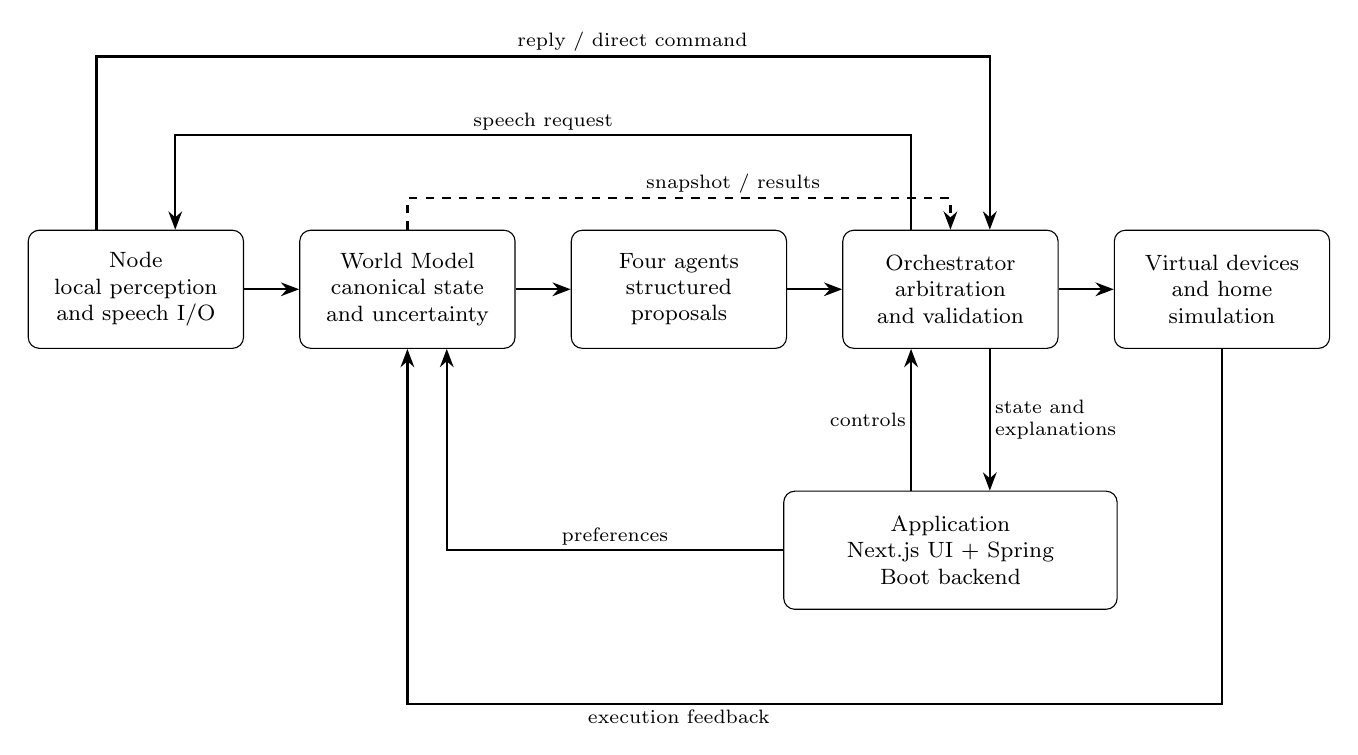
\begin{tikzpicture}[
box/.style={
draw,
rounded corners,
align=center,
text width=25mm,
minimum height=15mm,
font=\footnotesize
},
arr/.style={-{Stealth},thick},
edgeLabel/.style={
font=\scriptsize,
fill=white,
inner sep=1.5pt
},
node distance=7mm
]
\node[box] (node)
{Node\\local perception\\and speech I/O};

\node[box,right=of node] (world)
{World Model\\canonical state\\and uncertainty};

\node[box,right=of world] (agents)
{Four agents\\structured\\proposals};

\node[box,right=of agents] (central)
{Orchestrator\\arbitration\\and validation};

\node[box,right=of central] (devices)
{Virtual devices\\and home\\simulation};

\node[box,below=18mm of central,text width=40mm] (app)
{Application\\Next.js UI + Spring Boot backend};

\draw[arr] (node.east) -- (world.west);
\draw[arr] (world.east) -- (agents.west);
\draw[arr] (agents.east) -- (central.west);
\draw[arr] (central.east) -- (devices.west);

\draw[arr,dashed] (world.north) -- ++(0,4mm)
-| node[pos=0.30,above,edgeLabel] {snapshot / results}
(central.north);

\draw[arr] ([xshift=-5mm]central.north) -- ++(0,12mm)
-| node[pos=0.25,above,edgeLabel] {speech request}
([xshift=5mm]node.north);

\draw[arr] ([xshift=-5mm]node.north) -- ++(0,22mm)
-| node[pos=0.30,above,edgeLabel] {reply / direct command}
([xshift=5mm]central.north);

\draw[arr] (app.west)
-| node[pos=0.25,above,edgeLabel] {preferences}
([xshift=5mm]world.south);

\draw[arr] ([xshift=-5mm]app.north)
-- node[left,edgeLabel] {controls}
([xshift=-5mm]central.south);

\draw[arr] ([xshift=5mm]central.south)
-- node[right,edgeLabel,align=left] {state and\\explanations}
([xshift=5mm]app.north);

\coordinate (feedbackBottom) at ([yshift=-12mm]app.south);

\draw[arr] (devices.south) |- (feedbackBottom)
-| node[pos=0.25,below,edgeLabel] {execution feedback}
(world.south);
\end{tikzpicture}
\caption{Logical system interactions. Horizontal observation-to-action
flow is supplemented by voice, application, and device-feedback paths.
The dashed path supplies the Orchestrator with shared state and
correlated execution results. Crossings without junctions are not connections.}
\label{fig:flow}
\end{figure*}

Nodes send semantic events, the World Model publishes a
whole-home snapshot, agents produce proposals, and the
Orchestrator approves commands. Both the agents and Orchestrator
read the same accepted snapshot. Appliance adapters send execution
results to the World Model, which updates canonical device state
and forwards each correlated result and home revision to the
Orchestrator. MQTT is the planned Node event transport; local
service APIs connect state and application components.
The speech-request/reply route is bidirectional. The application backend sends preference updates to the World Model, which includes accepted values in the next versioned snapshot. Operator controls are sent to the Orchestrator. Routing details are configuration and do not change these responsibilities.

Table~\ref{tab:interfaces} defines the information required at
each boundary rather than fixing a legacy payload. The existing
prototype contract must be revised to represent occupancy
without tracks, uncertain identity, person position,
washer/light/curtain devices, and dialogue state. A new payload
is not treated as compatible merely because its old version
number is retained. Versioned JSON Schema and example messages
define exact field names, types, enumerations, units, and nullability
outside this summary table.

\begin{table*}[!t]
\caption{Required Interface Information}
\label{tab:interfaces}
\centering
\small
\begin{tabularx}{\textwidth}{
@{}L{0.19\textwidth}L{0.22\textwidth}Y@{}
}
\toprule
\textbf{Message} & \textbf{Direction}
& \textbf{Required information} \\
\midrule
Semantic event
& Node to World Model
& Version, event/source/session IDs, sequence, observation time,
room occupancy and confidence; available tracks, identity
source/confidence, position, posture/activity, audio context,
and brightness. \\

World snapshot
& World Model to Orchestrator
& Home revision and time; room occupancy/uncertainty; people
and positions; environment values and their observation times;
device states/capabilities; user preferences, routines,
and room relationships. \\

Agent proposal
& Agent to Orchestrator
& Agent and input-state version; proposed actions, restrictions,
soft scores, supporting observations, and deferred work. \\

Decision / command
& Orchestrator to adapter
& Plan/command IDs, input-state version, target device,
typed action/parameters, preconditions, and reason codes. \\

Execution result
& Adapter via World Model to Orchestrator
& Command ID, home revision,
accepted/rejected/completed/failed status, time,
observed device state, and failure reason when applicable. \\

Speech request / reply
& Orchestrator and Node
& Request ID, target room/Node, spoken text, reply expectation
and listening limit; playback completion; correlated reply
text/confidence or explicit no-response. Direct commands identify
their source and time. \\
\bottomrule
\end{tabularx}
\end{table*}

Messages are validated before use. Enumerations for uncertain
observations include an unknown state; unmeasured numeric values
are nullable rather than replaced with zero. Referenced IDs must
exist, timestamps have explicit time bases, and position
coordinates use a documented room frame. Room occupancy remains
separate from person tracking: an occupied room can have no
reliable person position. The World Model owns canonical home
revisions; issuing a command does not directly establish a new
observed device state.

\subsection{Node Perception and Local Fusion}
\label{sec:node}

The camera supplies face and pose evidence, tracking radar
supplies target locations/movement, and static-presence radar
supplies room-level presence. Independent components produce
timestamped observations; fusion associates compatible tracks
after coordinate calibration. Audio supplies context and
optional identity evidence. Sensor absence or poor visibility
reduces certainty rather than creating a false observation.

Rest inference compares a camera region with alternative text
descriptions, including resting and plausible non-resting
scenes, and checks pose evidence separately. The baseline
requires reliable, agreeing evidence over a configurable hold
duration. Insufficient evidence is unknown, not confirmed rest.
This conservative baseline can miss blanket-covered occupants
and must be evaluated accordingly. A transient loss of visual
evidence does not prove that a rest episode has ended.
Algorithm~\ref{alg:node} summarizes the local update. Activity and
identity are evaluated separately for each associated person track;
occupancy is evaluated once for the room, including presence without
a reliable track.

\begin{algorithm}[!tbp]
\caption{Local observation update}
\label{alg:node}
\footnotesize
\begin{algorithmic}[1]
\Require timestamped modality observations and local track history
\State Validate available inputs and associate compatible tracks

\If{reliable rest and lying evidence agree continuously}
  \State Update hold timer
  \If{the hold threshold has been reached}
    \State activity $\gets$ RESTING
  \Else
    \State activity $\gets$ UNKNOWN; retain candidate evidence
  \EndIf
\Else
  \State Clear candidate timer; report OTHER only with positive
  evidence, otherwise UNKNOWN
\EndIf

\If{a face confidently matches an enrolled resident}
  \State Bind identity to the associated track;
  source $\gets$ FACE
\ElsIf{an earlier binding has unambiguous continuity}
  \State Carry identity with reduced confidence and bounded lifetime
\Else
  \State Report unknown identity
\EndIf

\If{valid presence evidence indicates a person}
  \State occupancy $\gets$ OCCUPIED
\ElsIf{valid absence evidence persists for its confirmation period}
  \State occupancy $\gets$ EMPTY
\Else
  \State occupancy $\gets$ UNKNOWN
\EndIf

\State Publish changed observations or a periodic heartbeat
\end{algorithmic}
\end{algorithm}

For the single-occupant bedroom scenario, identity established
in the light may be retained through compatible track/presence
continuity after lights-off. This is historical association,
not radar identification. Confirmed exit, ambiguity, source
expiry, or additional occupants invalidate the binding.
A room entered in darkness without earlier identification
remains unknown. Face evidence is checked again after lights-on.
Raw frames/audio remain local; consented replay recordings are
stored separately from central messages.

\subsection{World Model and Replanning Triggers}
\label{sec:world}

For each source, the World Model tracks session, sequence,
observation time, and availability. Duplicate or reversed events
do not overwrite newer state. A source restart starts a new
tracked session rather than silently reusing its old sequence.
Missing heartbeats mark the source stale; they do not establish
an empty room. Stable activities and their durations are
aggregated without promoting image-text similarity directly
to a calibrated probability.

The Orchestrator validates each snapshot and detects changes
relevant to occupancy, confirmed activity, preferences, device
state, task progress, or dialogue. An unchanged heartbeat
refreshes availability without repeatedly invoking the LLM.
Closely spaced updates may be coalesced; a pending plan must be
rechecked before dispatch. Algorithm~\ref{alg:ingest} gives the
proposed acceptance flow.

\begin{algorithm}[!tbp]
\caption{Snapshot acceptance and trigger evaluation}
\label{alg:ingest}
\footnotesize
\begin{algorithmic}[1]
\Require snapshot $S$, stored state $W$, selected time base

\If{schema, references, or revision ordering are invalid}
  \State Record rejection; \Return
\EndIf

\If{$S$ is stale under the selected live/replay clock}
  \State Record stale input; \Return
\EndIf

\State Mark expired individual observations unavailable
\State Compare relevant fields of $S$ and $W$
\State $W \gets S$; store its accepted home revision

\If{a relevant state transition occurred}
  \State Enqueue or update a decision request
\EndIf
\end{algorithmic}
\end{algorithm}

Voice requests, replies, direct commands, and task timeouts are
additional triggers. A reply can therefore be handled without
waiting for a sensor change. The World Model also schedules source
expiry checks: if evidence expires without a new message, it marks
the affected state unknown, increments the home revision when state
changes, and publishes a new snapshot. The Orchestrator rechecks
freshness before every dispatch even if no update has arrived.
Unavailable identity or occupancy is preserved through the snapshot,
and actions requiring missing evidence are held rather than guessed.

\subsection{Agent Proposals and Appliance Policies}
\label{sec:agents}

The four agents read a common state version and produce
recommendations; none dispatches commands.
Table~\ref{tab:policies} specifies the primary scenario.
The occupancy-based rules in this table apply even before an
occupant is classified as resting. Optional activity-sensitive
refinements must not weaken them.

\begin{table*}[!t]
\caption{Primary Appliance Policies and Agent Outputs}
\label{tab:policies}
\centering
\small
\begin{tabularx}{\textwidth}{
@{}L{0.12\textwidth}L{0.25\textwidth}Y@{}
}
\toprule
\textbf{Agent} & \textbf{Inputs / output}
& \textbf{Processing policy} \\
\midrule
Cleaning
& Occupancy, routine and task progress;
output feasible rooms and deferred work
& Do not clean an occupied room; unknown occupancy is not
permission to clean. Returning to dock is a separate transit
action with the scenario's explicit exception. Retain unfinished
rooms and re-evaluate them after confirmed vacancy. \\

Noise
& Occupancy, activity, quiet preferences, adjacency, device modes;
output low-noise restrictions and soft preferences
& A manually started washer switches to supported low-noise
operation while a configured neighboring space is occupied.
Do not stop its cycle. Unknown occupancy does not justify
clearing protection. Restore an automation-modified mode only
after protection ends and no user override supersedes it. \\

Temperature
& Present residents, preferences, positions and AC capabilities;
output target and airflow direction
& Use the mean of the present identified residents' configured
preferred temperatures, mapped to a valid device setting.
Direct airflow toward the resident preferring the cooler target
when position/capability is available. Turn off after confirmed
vacancy; uncertainty alone does not prove vacancy. \\

Lighting
& Rest evidence, brightness/device state and dialogue history;
output question or conditional actions
& Ask once per confirmed rest episode. Close curtains and switch
lights off only for a valid affirmative reply; negative,
ambiguous or absent replies leave both unchanged. \\
\bottomrule
\end{tabularx}
\end{table*}

Per-resident quiet preferences add soft preferences for lower-noise
feasible modes during rest; they do not relax the mandatory occupied-room
vacuum or neighboring-washer policies. Missing identity/preferences or
position can disable personalization or airflow targeting while
preserving other feasible actions. The prototype does not infer
observed floor contamination. Cleaning history may prioritize
routine work without claiming a measured dirt level.

Each proposal records its agent, input-state version, typed
actions, hard restrictions, optional soft scores, evidence, and
reason codes. Lightweight learned scorers may supplement
ranking, disturbance assessment, or preference fit, but cannot
override mandatory constraints. If learning is added, use the
same feature extraction in training and runtime, features from
available snapshots/history only, and independent held-out days
or households. Compare with rule baselines using task-appropriate
metrics and missing-data tests. Dataset generation formulas and
measured performance are outside this specification milestone
and are not asserted as established results.

\subsection{Voice Dialogue and Direct Commands}
\label{sec:voice}

The lighting agent proposes a sleep-intent question when appropriate. The Orchestrator validates the proposal, manages the rest episode and question state, and sends the correlated speech request to the Node. A confirmed rest transition creates an episode. The question states are NOT\_ASKED, SPEAKING, AWAITING\_REPLY, ANSWERED, and EXPIRED. Confirmed rising/leaving closes the episode and invalidates its pending request. Unknown evidence alone does not end an episode or permit another question.

The Node plays the central text and reports playback completion.
It then listens for at most five seconds, transcribes detected
speech locally, and returns a correlated text/confidence or
no-response result. The central reply deadline accounts for
playback completion, the listening window, and a bounded
processing/delivery allowance. Playback is not treated as a
resident response. Per-request event ordering ensures playback
completion is processed before a subsequent reply.
Algorithm~\ref{alg:voice} handles the episode and its pending request.

\begin{algorithm}[!tbp]
\caption{One-question-per-rest dialogue}
\label{alg:voice}
\footnotesize
\begin{algorithmic}[1]
\Require episode $E$, state $Q$, correlated event, current time $t$

\If{$E$ is no longer active}
  \State Cancel pending request/actions; log cancellation; \Return
\EndIf

\If{$Q=$ NOT\_ASKED}
  \State Create request ID and playback deadline
  \State $Q\gets$ \Call{Transition}{SPEAKING}
  \State Send validated text and listening limit; \Return
\EndIf

\If{request ID or episode does not match}
  \State Ignore event; \Return
\EndIf

\If{$Q=$ SPEAKING}
  \If{playback deadline has expired}
    \State $Q\gets$ \Call{Transition}{EXPIRED}
  \ElsIf{matching playback completion arrives}
    \State Set reply deadline from playback completion
    \State $Q\gets$ \Call{Transition}{AWAITING\_REPLY}
  \EndIf
  \State \Return
\EndIf

\If{$Q\ne$ AWAITING\_REPLY}
  \State Ignore duplicate or obsolete event; \Return
\EndIf

\If{reply deadline expired or matching no-response arrives}
  \State $Q\gets$ \Call{Transition}{EXPIRED}
\ElsIf{a valid reply arrives before the deadline}
  \State Interpret text and confidence
  \State $Q\gets$ \Call{Transition}{ANSWERED}
  \If{reliably affirmative}
    \State Propose curtain-close/light-off for validation
  \EndIf
\EndIf
\end{algorithmic}
\end{algorithm}

The Transition operation stores the previous and new state, episode
and request IDs, time, and reason before returning the new state.
Timer events carry the same correlation IDs as replies. Playback
and reply deadlines therefore expire even without incoming speech.
Expiry, negative replies, and ambiguous replies leave lights and
curtains unchanged. Speech requests are validated for the target
Node and active episode before transmission. A confirmed episode
end cancels pending conditional actions; the command validator
checks that the episode remains valid before applying an
affirmative reply.

A wake phrase enables a direct command; earlier audio is
discarded inside the Node. The Node sends the recognized command
text centrally. The central service resolves its intended
room/device and requests clarification or holds if the target
is ambiguous. An authorized direct command supersedes automatic
plans but still passes policy and capability validation.
Turning the light on does not automatically reopen a curtain.
A manual override prevents conflicting automatic changes;
reset or an explicit release ends it in the prototype.

\subsection{Central Arbitration, Execution, and Trace}
\label{sec:central}

The central service evaluates four proposals against user
directives. Feasible candidate plans retain unmet goals.
The LLM receives a compact contextual summary and candidates
and returns a schema-validated plan selection with reason codes
and a brief explanation. It does not invent arbitrary appliance
API calls. Timeout, refusal, unavailable API, or invalid output
invokes the deterministic baseline or a safe hold. The same
policy validator checks both LLM and fallback results.
Algorithm~\ref{alg:central} separates selection, dispatch, and
asynchronous feedback.

\begin{algorithm}[!tbp]
\caption{Validated orchestration cycle}
\label{alg:central}
\footnotesize
\begin{algorithmic}[1]
\Require state $S$, directives $D$, task/dialogue history $H$

\State Collect four proposals based on $S$
\State Build feasible candidate plans; retain unmet goals
\State Initialize selection to unavailable

\If{LLM arbitration is enabled}
  \State Request bounded-time structured selection
\EndIf

\If{schema, candidate ID, or decision meaning is invalid}
  \State Set selection to unavailable
\EndIf

\If{selection is unavailable}
  \State Apply deterministic selection or choose HOLD
\EndIf

\If{selection is HOLD/NO\_OP or has no actions}
  \State Record reasons and retained tasks; \Return
\EndIf

\State Fetch latest relevant state; revalidate selected plan

\If{preconditions changed or required evidence expired}
  \State Record hold; request re-evaluation; \Return
\EndIf

\For{each selected action}
  \If{already issued or requires no device-state change}
    \State Record duplicate/no-change outcome
  \ElsIf{unauthorized, unsupported, or overridden}
    \State Record rejection
  \Else
    \State Dispatch with plan/command IDs; mark pending
  \EndIf
\EndFor

\State Record reasons/mode and retained tasks; \Return

\Statex \textbf{Asynchronous feedback handler:}
\State Receive World-Model-forwarded result; match command ID
\State Update pending status; complete only on completion evidence
\State Request re-evaluation using the updated home revision
\end{algorithmic}
\end{algorithm}

A command must match the target device's supported action, mode,
range, and parameter step. Automatic commands cannot bypass an
active manual override. A repeated event or repeated plan
selection must not create duplicate execution of the same
command. On failure or uncertain delivery, keep the task
unresolved; re-observe device state before retrying a
non-idempotent action. Partial multi-device success is recorded
per action rather than described as an atomic success. If a plan
declares action dependencies, dispatch a dependent action only after
its required predecessor succeeds; otherwise keep it pending or
record a blocked outcome. Dialogue requests use the validated Node
speech interface, and affirmative replies produce appliance
proposals that pass the same command validator.

Trace records include plan and command IDs, triggering
state/event, agent proposals, selected candidate, parameters,
validation results, arbitration mode, reasons, and execution
feedback. Deferred work is represented as remaining tasks,
not erased after a partial plan. A task becomes complete only
after matching completion feedback.

\subsection{Simulation, Replay, and Application}
\label{sec:sim}

The home simulation contains rooms, furniture, Node positions,
residents and virtual appliances. It visualizes vacuum
routes/dock, washer modes, AC target/airflow, lights and curtains,
together with the corresponding event, World Model state,
proposals, decision and feedback. Recorded, inferred and authored
information is labeled separately. Virtual devices implement
supported capabilities and return execution results; they do
not merely display intended commands as completed actions.

Live Node events, replayed sensor processing, and authored
scenarios enter compatible interfaces. Replay uses an explicit
scenario clock; freshness checks use that clock rather than
rejecting all recorded timestamps against wall time.
Reset clears scenario, task, pending-command and dialogue state.
Deterministic fallback with fixed input supports repeatable
policy testing; stochastic perception or LLM outputs are not
assumed bitwise identical.

The Next.js interface obtains views and controls through the
Spring Boot application backend. That backend stores validated
preferences and forwards authorized requests to central services;
it does not duplicate agent policies. The Spring Boot backend checks
a configured operator token for state-changing application requests;
central services separately check the application service credential
and registered Node source before accepting control input.
Credentials are configured outside source control.
Changed preferences are sent to the World Model and included
in the next versioned snapshot. Invalid values are rejected without
replacing the prior valid setting. Start/pause/reset/override controls
show their resulting state, and a rejected request or unavailable
service produces a visible error instead of an optimistic success
indication. Pausing automation does not imply stopping a running
washer. The interface displays observed device outcomes separately
from pending commands.

\subsection{Non-Functional Behavior and Verification}
\label{sec:verification}

Each sensor, model, transport and appliance boundary supports
a mock with the same logical interface. A missing source
preserves unknown state; provider failure displays degraded mode.
Raw media and API credentials are excluded from central messages
and traces. State-changing application and service endpoints check
their configured credentials; rejected requests have no control
effect. Trust in a registered Node is a controlled-demo assumption,
not proof of speaker identity. Public deployment requires stronger
resident authorization and encrypted communication.

Measure event-publication-to-decision and decision-to-display
latency on the recorded environment. The two-second
visible-decision goal is a target, not a measured result;
report LLM and fallback paths separately. Speech playback and
user response wait are measured separately. Confidence
thresholds, hold times, heartbeat/freshness periods and provider
timeouts are configurable and documented with the test build.

Acceptance tests cover occupied-room cleaning versus dock
transit, vacancy-triggered task resumption, washer low-noise
and permitted restoration, yes/no/ambiguous/no-response dialogue,
playback/reply timeouts, stale/duplicate replies,
direct commands and manual overrides, missing identity/presence,
stale/reversed input, invalid commands, partial device failures,
and LLM fallback. Tests record inputs, expected behavior,
actual output and trace evidence.
Planned tests are not reported as passing results.

\subsection{Primary Validation Scenario}
\label{sec:scenario}

Table~\ref{tab:scenario} summarizes the authored evening sequence.
It checks interactions among sensing, dialogue, policies, and
execution feedback rather than presenting measured performance.
For this authored fixture, the vacuum initially has a Room 2 task
followed by a preset dock-return task. The Room 1 routine becomes
due at t1; thus t0 does not imply that docking was chosen over
another available cleaning task. These are scenario initial
conditions rather than general scheduling rules.

\begin{table*}[!t]
\caption{Scripted Evening Scenario: Residents A and B
Prefer 24 and 26$^\circ$C}
\label{tab:scenario}
\centering
\small
\begin{tabularx}{\textwidth}{
@{}L{0.04\textwidth}L{0.40\textwidth}Y@{}
}
\toprule
\textbf{Step} & \textbf{Observation / event}
& \textbf{Expected behavior} \\
\midrule
t0
& Washer running; B watches TV; Room 2 finishes and preset
dock return begins.
& Living-room AC target 26$^\circ$C toward B; dock-return
transit through living room permitted. \\

t1
& Room 1 cleaning becomes due; A enters bright Room 1
and is identified.
& Defer Room 1 cleaning; neighboring washer low-noise;
Room 1 AC target 24$^\circ$C. \\

t2
& Reliable lying/rest evidence persists.
& Create one rest episode and ask one sleep-intent question. \\

t3
& A reliably answers yes to that question.
& Validate curtain-close/light-off; retain identity only
under documented continuity conditions. \\

t4
& Room is dark and static-presence evidence continues.
& Maintain occupancy and protection; do not claim visually
proven sleep or repeat the question. \\

t5
& Wake phrase followed by a request to turn on the light.
& Validate direct command; turn light on, leave curtain
unchanged, and recheck identity. \\

t6
& Room 1 becomes confirmed empty.
& Re-evaluate deferred cleaning; Room 1 AC off; restore
washer mode only when protection and override conditions permit. \\

t7
& A joins B on the living-room sofa.
& AC target 25$^\circ$C toward A; ordinary sitting does
not trigger a sleep question. \\
\bottomrule
\end{tabularx}
\end{table*}

Only Room 1 uses the physical surrogate Node; other room
observations are authored or simulated and labeled accordingly.
Negative, ambiguous, and no-response branches leave lighting
unchanged. This scenario is an acceptance fixture, not evidence
that all components have already passed evaluation.

Table~\ref{tab:trace} maps all requirements to their specifications
and planned verification. Optional learning is evaluated only
if included; the baseline scenario does not depend on it.

\begin{table*}[!t]
\caption{Requirement-to-Specification and Verification Mapping}
\label{tab:trace}
\centering
\footnotesize
\begin{tabularx}{\textwidth}{
@{}L{0.12\textwidth}L{0.23\textwidth}Y@{}
}
\toprule
\textbf{Requirement} & \textbf{Specification}
& \textbf{Planned verification} \\
\midrule
R-01
& Secs.~\ref{sec:agents}, \ref{sec:central}
& Occupied-room block, dock transit, deferred-goal retention
and vacancy-triggered completion. \\

R-02
& Secs.~\ref{sec:agents}, \ref{sec:voice}
& Washer protection and yes/no/ambiguous/no-response
light/curtain branches. \\

R-03
& Secs.~\ref{sec:central}, \ref{sec:sim}
& Inspect states/reasons and exercise start, pause,
reset and override. \\

R-04--R-05
& Sec.~\ref{sec:node}
& Run independent components/mocks without changing
boundary semantics. \\

R-06
& Sec.~\ref{sec:node}; Alg.~\ref{alg:node}
& Persistent rest evidence, occlusion, false triggers
and unknown identity. \\

R-07
& Secs.~\ref{sec:node}, \ref{sec:voice}
& Acoustic labels, speech gating, ambiguous audio
and local-only processing. \\

R-08--R-09
& Sec.~\ref{sec:node}
& Motionless presence, track loss, identity expiry
and bright--dark--bright transitions. \\

R-10
& Secs.~\ref{sec:node}, \ref{sec:verification}
& Inspect central messages/traces for raw media;
separate consented recordings. \\

R-11
& Sec.~\ref{sec:flow}
& Valid/invalid event cases, versions, references
and unknown/null semantics. \\

R-12
& Sec.~\ref{sec:world}
& Multiple sources, stale/duplicate/reversed observations
and source restart. \\

R-13--R-14
& Secs.~\ref{sec:flow}, \ref{sec:world}
& Versioned state preserves occupancy/identity/activity
uncertainty. \\

R-15
& Sec.~\ref{sec:agents}
& Four proposals share a state version and contain
typed recommendations. \\

R-16--R-17
& Sec.~\ref{sec:central}
& Invalid LLM selection, capability failure
and direct-command precedence. \\

R-18--R-19
& Secs.~\ref{sec:world}, \ref{sec:central}
& Meaningful triggers, pre-dispatch recheck,
trace and feedback correlation. \\

R-20
& Sec.~\ref{sec:agents}
& If learning is included, compare with baselines
on held-out data. \\

R-21--R-23
& Sec.~\ref{sec:sim}
& Visible pipeline, compatible input paths,
explicit replay clock and labeled origins. \\

R-24
& Sec.~\ref{sec:verification}
& Missing-source mocks and visibly degraded LLM fallback. \\

R-25
& Sec.~\ref{sec:verification}
& Measured latency, reset/replay and recorded environment. \\

R-26
& Sec.~\ref{sec:verification}
& Malformed/unauthorized input, invalid commands
and acceptance evidence. \\

R-27
& Sec.~\ref{sec:voice}; Alg.~\ref{alg:voice}
& Bounded listening, no-response, duplicate/late replies
and direct commands. \\

R-28
& Sec.~\ref{sec:sim}
& Preference validation, propagation, operator controls
and error display. \\
\bottomrule
\end{tabularx}
\end{table*}

\section*{Scope and Verification Status}

This document specifies an academic prototype rather than
LG-approved product requirements or completed experimental
results. The baseline prioritizes the limited end-to-end
scenario and deterministic verification; learned improvements
remain optional. Hardware performance, recognition accuracy,
integration compatibility and latency must be measured.
Submitted source revisions, verified setup details and
resulting evidence will be maintained with the project.

\FloatBarrier
\begin{thebibliography}{20}

\bibitem{lg2024}
LG Electronics,
``LG to Introduce Exciting Vision for Future Living with
LG AI Home Innovations at IFA 2024,''
LG USA Press Release, Sep. 5, 2024.
[Online]. Available:
\url{https://www.lg.com/us/lg-to-introduce-exciting-vision-for-future-living-with-lg-ai-home-innovations-at-ifa-2024}.

\bibitem{esphome_ld2450}
ESPHome,
``LD2450 Sensor,''
ESPHome Documentation.
[Online]. Available:
\url{https://esphome.io/components/sensor/ld2450/}.

\bibitem{hlk_ld2410c}
Shenzhen Hi-Link Electronic Co., Ltd.,
``HLK-LD2410C Human Presence Motion Module User Manual,''
ver. V1.00, Nov. 7, 2022.
[Online]. Available:
\url{https://www.hestore.eu/en/prod_getfile.php?id=17796}
(distributor-hosted manufacturer manual).

\bibitem{mediapipe}
Google,
``MediaPipe Solutions Guide,''
Google AI Edge Documentation.
[Online]. Available:
\url{https://developers.google.com/mediapipe}.

\bibitem{blazepose}
V. Bazarevsky, I. Grishchenko, K. Raveendran, T. Zhu,
F. Zhang, and M. Grundmann,
``BlazePose: On-device real-time body pose tracking,''
arXiv preprint arXiv:2006.10204, 2020.

\bibitem{arcface}
J. Deng, J. Guo, N. Xue, and S. Zafeiriou,
``ArcFace: Additive angular margin loss for deep face recognition,''
in \emph{Proc. IEEE/CVF Conf. Computer Vision and
Pattern Recognition (CVPR)}, 2019.

\bibitem{mobileclip}
P. K. A. Vasu, H. Pouransari, F. Faghri,
R. Vemulapalli, and O. Tuzel,
``MobileCLIP: Fast image-text models through multi-modal
reinforced training,''
in \emph{Proc. IEEE/CVF Conf. Computer Vision and
Pattern Recognition (CVPR)}, 2024.

\bibitem{clip}
A. Radford \emph{et al.},
``Learning transferable visual models from natural
language supervision,''
in \emph{Proc. Int. Conf. Machine Learning (ICML)}, 2021.

\bibitem{yamnet}
Google,
``YAMNet: audio event classifier trained on AudioSet,''
TensorFlow Models repository.
[Online]. Available:
\url{https://github.com/tensorflow/models/tree/master/research/audioset/yamnet}.

\bibitem{whisper}
A. Radford, J. W. Kim, T. Xu, G. Brockman,
C. McLeavey, and I. Sutskever,
``Robust speech recognition via large-scale weak supervision,''
in \emph{Proc. Int. Conf. Machine Learning (ICML)}, 2023.

\bibitem{mqtt}
OASIS,
``MQTT Version 5.0,''
OASIS Standard, 2019.
[Online]. Available:
\url{https://docs.oasis-open.org/mqtt/mqtt/v5.0/mqtt-v5.0.html}.

\bibitem{mosquitto}
Eclipse Foundation,
``Eclipse Mosquitto: an open source MQTT broker.''
[Online]. Available:
\url{https://mosquitto.org}.

\bibitem{pydantic}
Pydantic,
``Pydantic Documentation.''
[Online]. Available:
\url{https://docs.pydantic.dev}.

\bibitem{openai_struct}
OpenAI,
``Structured Outputs,''
OpenAI Platform Documentation.
[Online]. Available:
\url{https://platform.openai.com/docs/guides/structured-outputs}.

\bibitem{lightgbm}
G. Ke \emph{et al.},
``LightGBM: A highly efficient gradient boosting decision tree,''
in \emph{Advances in Neural Information Processing Systems
(NIPS)}, 2017.

\bibitem{sklearn}
F. Pedregosa \emph{et al.},
``Scikit-learn: Machine learning in Python,''
\emph{J. Machine Learning Research},
vol. 12, pp. 2825--2830, 2011.

\end{thebibliography}

\end{document}